\vspace{-1mm}
\section{Related Work}
\label{sec:related_works}
\vspace{-1mm}
\textbf{Large Language Model Compression:}
%
LLMs in general contain billion-scale parameters. Applying conventional model compression methods for LLMs is unfeasible as they necessitate resource-intensive retraining. Given that, post-training methods that avoid retraining in the compression process have been proposed. 
%
In general, these methods can be grouped into four categories: unstructured pruning, structured pruning, quantization, and low-rank approximation.
%
Specifically, unstructured pruning methods~\citep{DBLP:conf/icml/FrantarA23} set the individual weights of an LLM to zero without changing its shape. However, irregular sparsification of unstructured pruning is difficult to achieve the desired speedup or memory saving.
%and can only demonstrate its best efficiency on certain hardware architecture. 
%
Unlike unstructured pruning, structured pruning methods~\citep{DBLP:conf/nips/MaFW23, DBLP:conf/iclr/AshkboosCNHH24, DBLP:journals/corr/abs-2406-10594} remove entire channels or other structured components from LLMs, making them easier to implement on hardware. One notable contribution is LLM-Pruner~\citep{DBLP:conf/nips/MaFW23}, which groups weight matrices based on their dependency and assigns the pruning ratio to each group based on the estimated importance. 
%However, due to the great modification of the weight matrix, it suffers from accuracy degradation especially under high compression ratios.
%
% SliceGPT~\citep{DBLP:conf/iclr/AshkboosCNHH24} and BlockPruner~\citep{DBLP:journals/corr/abs-2406-10594} have been proposed with better compression performance. 
Quantization methods~\citep{DBLP:journals/corr/abs-2405-04532} compress models by reducing the precision of weight matrices of the LLM. However, similar to unstructured pruning, quantization is also difficult to achieve the desired inference speedup due to the lack of hardware support and efficient kernels for low-precision computation~\citep{DBLP:journals/corr/abs-2405-04532}.
%
Recent studies including PB-LLM~\citep{DBLP:conf/iclr/YuanSD24} and BiLLM~\citep{DBLP:conf/icml/HuangLQLZ0M024} push the frontier to 1-bit quantization. Nevertheless, these approaches often lead to severe accuracy degradation.
%, indicating that 1-bit quantization remains a challenging aspect of LLM compression.


\begin{figure*}[t]
\centering
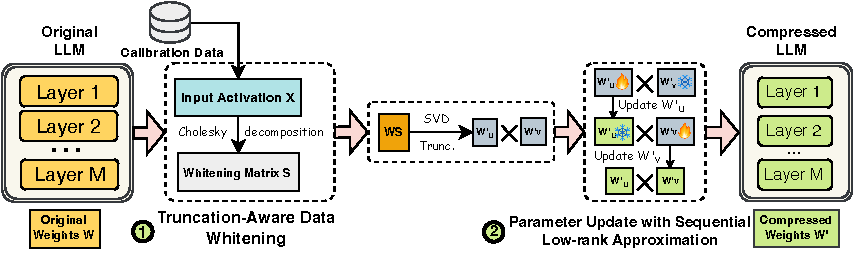
\includegraphics[width=1\textwidth]{Figures/Framework.pdf}
\vspace{-3mm}
\caption{Overview of \sysname.}
\vspace{-3mm}
\label{fig:framework}
\end{figure*}

\textbf{SVD for Language Model Compression:} Singular Value Decomposition (SVD) is a widely used low-rank approximation technique to reduce matrix size by approximating a matrix with two smaller low-ranking matrices~\citep{GOLUB1987317}. Given that, SVD is commonly used for model compression. 
%
For instance, DRONE~\citep{DBLP:conf/nips/ChenYDH21}  achieves optimal SVD compression for small language models such as BERT. However, during SVD compression, DRONE caches all the input activations, making it challenging for LLM compression due to excessive memory usage.
%, leading to the proposal of many new methods.
% %
% AAFM~\citep{DBLP:conf/aaai/YuW23} dynamically identifies the compressed model architecture and selectively compresses the output features of individual linear layers instead of the model weights. 
% %
% LoSparse~\citep{DBLP:conf/icml/LiYZLHCZ23} compresses the weight matrix by the sum of a low-rank matrix and a sparse matrix.
% %
% ARS~\citep{DBLP:conf/naacl/GaoHHSJ24} dynamically allocates the rank of the SVD compression based on the importance of weights in the LLM.
%
For LLMs, directly applying SVD on the weight matrix without considering the importance of the weights leads to a large compression loss. To address this issue, \citet{DBLP:conf/iclr/HsuHCLSJ22} propose FWSVD, which introduces Fisher information to weigh the importance of parameters. However, FWSVD requires a complex gradient calculation that demands substantial computing and memory resources for LLM compression. 
%
Another issue of directly applying SVD is that the distribution of activation can affect the compression loss. To address it, \citet{DBLP:journals/corr/abs-2312-05821} propose ASVD, which scales the weight matrix by a diagonal matrix that normalizes the impact of input channels on the weights.
%
However, both FWSVD and ASVD do not establish a direct relationship between singular values and compression loss. As a consequence, truncating the smaller singular values may lead to higher compression loss. Moreover, as compression ratio increases, it becomes necessary to update the compressed weights for accuracy recovery. However, both FWSVD and ASVD do not take it into consideration, and thus incur severe accuracy degradation under high compression ratios.